% \documentclass[11pt,twoside]{book} %纸质版用twoside
\documentclass[12pt,oneside]{book} %电子版用oneside
\usepackage{setspace}

% \documentclass{article}

%%%%%%%%%%%%%%%%%%%%%%%%%%%%%%%%%%%%%%%%%%%%%%%%%%
%%%%%%%%%%%%%%%%%%%%% preamble %%%%%%%%%%%%%%%%%%%
%%%%%%%%%%%%%%%%%%%%%%%%%%%%%%%%%%%%%%%%%%%%%%%%%%

\usepackage[mono=false]{libertine} % new linux font, ignore mono

\usepackage{luatex85}

%\renewcommand{\baselinestretch}{1.05}
\usepackage{amsmath,amsthm,amssymb,mathrsfs,amsfonts,dsfont}
\usepackage{epsfig,graphicx}
\usepackage{tabularx}
\usepackage{blkarray}
\usepackage{slashed}
\usepackage{color}
\usepackage{listings}
\usepackage{caption}
% \usepackage{fullpage}
\usepackage{lipsum} % provides dummy text for testing
\usepackage[toc,title,titletoc,header]{appendix}
\usepackage{minitoc}
\usepackage{color}
\usepackage{multicol} % two-col ToC
\usepackage{bm}
\usepackage{imakeidx} % before hyperref
\usepackage{hyperref}
\usepackage{indentfirst}
\setlength{\parindent}{2em}


% link colors settings
\hypersetup{
    colorlinks=true,
    citecolor=magenta,
    linkcolor=blue,
    filecolor=green,      
    urlcolor=cyan,
    % hypertexnames=false,
}
\usepackage[capitalise]{cleveref}
\usepackage{subcaption}
\usepackage{enumitem}
\usepackage{mathtools}
\usepackage{physics}
\usepackage[linesnumbered,ruled,vlined,algosection]{algorithm2e}
\SetCommentSty{textsf}
\usepackage{epigraph}
\epigraphwidth=1.0\linewidth
\epigraphrule=0pt

% adjust margin
\usepackage[margin=2.3cm]{geometry}
\headheight13.6pt


\usepackage{graphicx}
\usepackage[justification=centering]{caption} % 图注居中
\usepackage{setspace}
\usepackage{geometry}
\usepackage{float}
\usepackage{hyperref}
\usepackage[utf8]{inputenc}
\usepackage[english]{babel}
\usepackage{framed}


\newcommand{\HRule}[1]{\rule{\linewidth}{#1}}





\setstretch{1.2}
% \geometry{
%     textheight=9in,
%     textwidth=5.5in,
%     top=1in,
%     headheight=12pt,
%     headsep=25pt,
%     footskip=30pt
% }





%%%%%%%%%%%%%%%% thmtools %%%%%%%%%%%%%%%%%%%%%

\usepackage{thmtools}
\usepackage[dvipsnames]{xcolor}
\usepackage[most]{tcolorbox}
\usepackage{enumerate}

\colorlet{LightGreen}{Green!15} %def
\colorlet{LightBlue}{Blue!15} %thm
\colorlet{LightOrange}{Orange!15} %lem
\colorlet{LightGray}{Gray!15}  %prop
\colorlet{LightRed}{Red!40} %cor
\colorlet{LightYellow}{Yellow!15} %exa


% \newtcbtheorem[
%   number within = chapter % 按每个 chapter 分别编号
% ]{definition% 环境名
% }{Definition% 这个参数可以设成“定理”“引理”“推论”等,编号就会变成“定理 1.1”“引理 1.1”“推论 1.1”等
% }{
%   attach title to upper = \par\vspace{1ex}, % 不要单独的标题栏,定理名完了之后分段,加上适量空白
%   separator sign = \quad, % 定理编号和定理名字之间用什么分隔;默认是冒号
%   sharp corners, % 直角;默认是圆角
%   enhanced jigsaw, frame hidden, % 隐藏 tcb 边框
%   colback = LightGreen, % 背景色
%   coltitle = blue!20!cyan!80!black, % 标题(定理编号和名字)的颜色
%   fonttitle = \sffamily\small, % 标题(定理编号和名字)的字体
%   description font = \normalsize, % 定理名字的字体
%   fontupper = \normalfont, % box 内的字体
% }{def% label 前缀
% }

\newtcbtheorem[
  auto counter,number within = chapter % 按每个 chapter 分别编号
]{definition% 环境名
}{Definition% 这个参数可以设成“定理”“引理”“推论”等,编号就会变成“定理 1.1”“引理 1.1”“推论 1.1”等
}{
  sharp corners, % 直角;默认是圆角
  colback=Green!5,
  colframe=Green!50!black,
  fonttitle=\sffamily\small
}{def% label 前缀
}


% 计数器设置
\makeatletter
\renewcommand\theHtcb@cnt@definition{\thechapter.\arabic{tcb@cnt@definition}}
\makeatother

\newtcbtheorem[
  auto counter,number within = chapter % 按每个 chapter 分别编号
]{theorem% 环境名
}{Theorem% 这个参数可以设成“定理”“引理”“推论”等,编号就会变成“定理 1.1”“引理 1.1”“推论 1.1”等
}{
  sharp corners, % 直角;默认是圆角
  colback=yellow!10,
  colframe=yellow!50!black,
  fonttitle=\sffamily\small
}{thm% label 前缀
}
% 计数器设置
\makeatletter
\renewcommand\theHtcb@cnt@theorem{\thechapter.\arabic{tcb@cnt@theorem}}
\makeatother

\newtcbtheorem[
  auto counter,number within = chapter % 按每个 chapter 分别编号
]{proposition% 环境名
}{Proposition% 这个参数可以设成“定理”“引理”“推论”等,编号就会变成“定理 1.1”“引理 1.1”“推论 1.1”等
}{
  sharp corners, % 直角;默认是圆角
  colback=Red!5,
  colframe=Red!50!black,
  fonttitle=\sffamily\small
}{prop% label 前缀
}
% 计数器设置
\makeatletter
\renewcommand\theHtcb@cnt@proposition{\thechapter.\arabic{tcb@cnt@proposition}}
\makeatother

\newtcbtheorem[
  auto counter,number within = chapter % 按每个 chapter 分别编号
]{corollary% 环境名
}{Corollary% 这个参数可以设成“定理”“引理”“推论”等,编号就会变成“定理 1.1”“引理 1.1”“推论 1.1”等
}{
  sharp corners, % 直角;默认是圆角
  colback=Blue!5,
  colframe=Blue!50!black,
  fonttitle=\sffamily\small
}{cor% label 前缀
}

% 计数器设置
\makeatletter
\renewcommand\theHtcb@cnt@corollary{\thechapter.\arabic{tcb@cnt@corollary}}
\makeatother

\newtcbtheorem[
  auto counter,number within = chapter % 按每个 chapter 分别编号
]{lemma% 环境名
}{Lemma% 这个参数可以设成“定理”“引理”“推论”等,编号就会变成“定理 1.1”“引理 1.1”“推论 1.1”等
}{
  sharp corners, % 直角;默认是圆角
  colback=Gray!10,
  colframe=Gray!50!black,
  fonttitle=\sffamily\small
}{lem% label 前缀
}

% 计数器设置
\makeatletter
\renewcommand\theHtcb@cnt@lemma{\thechapter.\arabic{tcb@cnt@lemma}}
\makeatother


\newtcbtheorem[
  auto counter,number within = chapter % 按每个 chapter 分别编号
]{example}
{Example}%
  {
    enhanced, breakable,
    colback = white, colframe = purple, colbacktitle = purple,
    attach boxed title to top left = {yshift = -2mm, xshift = 5mm},
    boxed title style = {sharp corners},
    fonttitle=\sffamily\small
  }
{exa}

% 计数器设置
\makeatletter
\renewcommand\theHtcb@cnt@example{\thechapter.\arabic{tcb@cnt@example}}
\makeatother


\newtcbtheorem[
  auto counter,number within = chapter % 按每个 chapter 分别编号
]{exercise}
{Exercise}%
  {
    enhanced, breakable,
    colback = white, colframe = cyan, colbacktitle = cyan,
    attach boxed title to top left = {yshift = -2mm, xshift = 5mm},
    boxed title style = {sharp corners},
    fonttitle=\sffamily\small
  }
{exer}

% 计数器设置
\makeatletter
\renewcommand\theHtcb@cnt@exercise{\thechapter.\arabic{tcb@cnt@exercise}}
\makeatother


% \declaretheorem[numberwithin=chapter,shaded={rulecolor=LightGreen,
% rulewidth=2pt,bgcolor=LightGreen,
% textwidth=12em}]{definition}

\usepackage{changepage}
\newenvironment{remark}{\underline{\textbf{Remark.}}}{\par}

\newenvironment{proofsolution}
    {\renewcommand\qedsymbol{$\square$}\color{blue}\begin{adjustwidth}{0em}{2em}\begin{proof}[\textit Proof.~]}
    {\end{proof}\end{adjustwidth}}


%%%%%%%%%%%%%%%% index %%%%%%%%%%%%%%%%%%%%%
\begin{filecontents}{index.ist}
% https://tex.stackexchange.com/questions/65247/index-with-an-initial-letter-of-the-group
headings_flag 1
heading_prefix "{\\centering\\large \\textbf{"
heading_suffix "}}\\nopagebreak\n"
delim_0 "\\nobreak\\dotfill"
\end{filecontents}
\newcommand{\myindex}[1]{\index{#1} \emph{#1}}
\makeindex[columns=3, intoc, title=Alphabetical Index, options= -s index.ist]
%%%%%%%%%%%%%%%% index %%%%%%%%%%%%%%%%%%%%%

%%%%%%%%%%%%%%%% ToC %%%%%%%%%%%%%%%%%%%%%
% Link Chapter title to ToC: https://tex.stackexchange.com/questions/32495/linking-the-section-text-to-the-toc
\usepackage[explicit]{titlesec}
\titleformat{\chapter}[display]
  {\normalfont\huge\bfseries}{\chaptertitlename\ {\thechapter}}{20pt}{\hyperlink{chap-\thechapter}{\Huge#1}
\addtocontents{toc}{\protect\hypertarget{chap-\thechapter}{}}}
\titleformat{name=\chapter,numberless}
  {\normalfont\huge\bfseries}{}{-20pt}{\Huge#1}

%%%%%%%%%%%%%%%%%%% fancyhdr %%%%%%%%%%%%%%%%%
\usepackage{fancyhdr}
\pagestyle{fancy} % enable fancy page style
\renewcommand{\headrulewidth}{0.0pt} % comment if you want the rule
\fancyhf{} % clear header and footer
\fancyhead[lo,le]{\leftmark}
\fancyhead[re,ro]{\rightmark}
\fancyfoot[CE,CO]{\hyperref[toc-contents]{\thepage}}

% https://tex.stackexchange.com/questions/550520/making-each-page-number-link-back-to-beginning-of-chapter-or-section
\makeatletter
\def\chaptermark#1{\markboth{\protect\hyper@linkstart{link}{\@currentHref}{Chapter \thechapter ~ #1}\protect\hyper@linkend}{}}
\def\sectionmark#1{\markright{\protect\hyper@linkstart{link}{\@currentHref}{\thesection ~ #1}\protect\hyper@linkend}}
\makeatother
%%%%%%%%%%%%%%%%%%% fancyhdr %%%%%%%%%%%%%%%%%


%%%%%%%%%%%%%%%%%%% biblatex %%%%%%%%%%%%%%%%%
\usepackage[doi=false,url=false,isbn=false,style=alphabetic,backend=biber,backref=true]{biblatex}
\addbibresource{bib.bib}

\newbibmacro{string+doiurlisbn}[1]{%
  \iffieldundef{doi}{%
    \iffieldundef{url}{%
      \iffieldundef{isbn}{%
        \iffieldundef{issn}{%
          #1%
        }{%
          \href{http://books.google.com/books?vid=ISSN\thefield{issn}}{#1}%
        }%
      }{%
        \href{http://books.google.com/books?vid=ISBN\thefield{isbn}}{#1}%
      }%
    }{%
      \href{\thefield{url}}{#1}%
    }%
  }{%
    \href{http://dx.doi.org/\thefield{doi}}{#1}%
  }%
}

% https://tex.stackexchange.com/questions/94089/remove-quotes-from-inbook-reference-title-with-biblatex
\DeclareFieldFormat[article,incollection,inproceedings,book,misc]{title}{\usebibmacro{string+doiurlisbn}{\mkbibemph{#1}}}
% https://tex.stackexchange.com/questions/454672/biblatex-journal-name-non-italic
\DeclareFieldFormat{journaltitle}{#1\isdot}
\DeclareFieldFormat{booktitle}{#1\isdot}
% https://tex.stackexchange.com/questions/10682/suppress-in-biblatex
\renewbibmacro{in:}{}
% add video field: https://tex.stackexchange.com/questions/111846/biblatex-2-custom-fields-only-one-is-working
\DeclareSourcemap{
    \maps[datatype=bibtex]{
      \map{
        \step[fieldsource=video]
        \step[fieldset=usera,origfieldval]
    }
  }
}
\DeclareFieldFormat{usera}{\href{#1}{\textsc{Online video}}}
\AtEveryBibitem{
    \csappto{blx@bbx@\thefield{entrytype}}{% put at end of entry
        \iffieldundef{usera}{}{\space \printfield{usera}}
    }
}


%%%%%%%%%%%%%%%%%%%%%%%notations%%%%%%%%%%%%%%%%%%%%%%%%%%%%%%
\newcommand{\F}{\ensuremath{\mathbb{F}}}
\newcommand{\C}{\ensuremath{\mathbb{C}}} 
\newcommand{\R}{\ensuremath{\mathbb{R}}}
\newcommand{\J}{\ensuremath{\mathbb{J}}}
\newcommand{\Q}{\ensuremath{\mathbb{Q}}}
\newcommand{\Z}{\ensuremath{\mathbb{Z}}}
\newcommand{\N}{\ensuremath{\mathbb{N}}}
\newcommand{\K}{\ensuremath{\mathbb{K}}}
\newcommand{\Zo}{\ensuremath{\mathbb{Z}_{\geqslant 0}}} % 非负整数集
\newcommand{\Zi}{\ensuremath{\mathbb{Z}_{\geqslant 1}}} % 正整数集
\newcommand{\id}{\mathrm{id}}
\newcommand{\im}{\mathrm{im}\,}                         % 映射的像
\newcommand{\leqs}{\leqslant}
\newcommand{\geqs}{\geqslant}
\newcommand{\ci}{\mathrm{i}}
\newcommand{\hH}{\mathscr{H}}
\newcommand{\hK}{\mathscr{K}}
\newcommand{\inner}[2]{\langle#1,#2\rangle}

%%%%%%%%%%%%%%%%%%% biblatex %%%%%%%%%%%%%%%%%

%%%%%%%%%%%%%%%%%%%%% glossaries %%%%%%%%%%%%%%%%%
% !TEX root = ./notes_template.tex
% \usepackage[style=super]{glossaries}
% https://www.overleaf.com/learn/latex/Glossaries
\usepackage[style=super,toc,acronym]{glossaries}
\setlength{\glsdescwidth}{1\linewidth}
\makeglossaries

\renewcommand\glossaryname{List of Abbreviations and Symbols}

\newglossaryentry{Q2}{name={$Q_2(f)$},
%sort=Q2,
description={Two-side (bounded) error quantum query complexity}}

\newglossaryentry{real_number}{name={$\mathbb{R}$},description={Real number}}

% \newglossaryentry{gcd}{name={gcd},description={greatest common divisor}}

\newacronym{gcd}{GCD}{Greatest Common Divisor}


\newglossaryentry{svm}{name={SVM},description={Support Vector Machine}}

\newglossaryentry{gd}{name={GD},description={Gradient Descent}}

\newglossaryentry{qft}{name={QFT},description={Quantum Field Theory}}

\newglossaryentry{qm}{name={QM},description={Quantum Mechanics}}

\newglossaryentry{v}{name={$\vec{v}$},description={a vector}}

% physics
\newglossaryentry{hamiltonian}{name={$\hat{H}$},description={Hamiltonian}}

\newglossaryentry{lagrangian}{name={$L$},description={Lagrangian}}
%%%%%%%%%%%%%%%%%%%%% glossaries %%%%%%%%%%%%%%%%%

%%%%%%%%%%%%%%%%%%%%% glossaries-extra %%%%%%%%%%%%%%%%%
% \usepackage[record,abbreviations,symbols,stylemods={list,tree,mcols}]{glossaries-extra}
%%%%%%%%%%%%%%%%%%%%% glossaries-extra %%%%%%%%%%%%%%%%%


% !TEX root = ./notes_template.tex

%%%%%%%%%%%%%%%%%%%%%%%%%%%%%%%%%%%%
%%%%%%%%%%%%%%%%%%%%%%%%%%%%%%%%%%%%
% math
\let\iff\relax
\newcommand{\iff}{\text{ iff }}
\newcommand{\OPT}{\textup{OPT}}

% physics
\newcommand{\acreation}{a^\dagger}



%%%%%%%%%%%%%%%%%%%%%%%%%%%%%%%%%%%%%%%%%%%%%%%%%%
%%%%%%%%%%%%%%%% begin of document %%%%%%%%%%%%%%%
%%%%%%%%%%%%%%%%%%%%%%%%%%%%%%%%%%%%%%%%%%%%%%%%%%

\begin{document}

\title{\bf \huge Study Notes of Numerical Optimization}
\author{Pei Zhong}
\date{Update on \today}

\maketitle

% \newpage
% \let\cleardoublepag\clearpage

\tableofcontents

\begin{spacing}{1}

%%%%%%%%%%%%%%update progress%%%%%%%%%%
\chapter*{Update progress}
\begin{itemize}
    \item {writing ch\ref{chp:Convex Optimization}... \hfill 2023.10.20}
\end{itemize}


%%%%%%%%%%%%%%update progress end%%%%%%%%




%%%%%%%%%%%%%%%preface%%%%%%%%%%%%%
\chapter*{Preface}


Notes mainly refer to the following resources:
\begin{itemize}
    \item \href{https://www-labs.iro.umontreal.ca/~grabus/courses/ift6760a-w20.html}{lecture notes from course "Matrix and tensor factorization techniques for machine learning"}
    \item \href{https://web.stanford.edu/class/cs168/}{lecture notes from course "The Modern Algorithmic Toolbox"}
\end{itemize}

\par

all the codes in the notes are completed by python. You can get the codes in the following website:
\begin{itemize}
    \item -
\end{itemize}


%%%%%%%%%%%%%preface end%%%%%%%%%%%%%

\part{Fundamental Concepts of Optimization}
%%%%%%%%%%%%%ch1 convex%%%%%%%%%%%%%%
\chapter{Convex Optimization}\label{chp:Convex Optimization}


\textit{"The great watershed in Optimization is not 
between linearity and nonlinearity, but convexity and nonconvexity. "}

%%%%%%%%%%%%ch1 section1%%%%%%%%%%%
\section{General Convex Optimization Problems}
\begin{definition}{
    (Convex Set) % 定理的名字
  }{% label
  }
    {
        a set \ $\Omega\in \R^n$ is convex if 
         \begin{equation}
            \forall x,y \in \Omega, t\in [0,1]: x+t(y-x)\in \Omega. 
         \end{equation}


        
    }
\end{definition}


\begin{remark}
    This definition is equivalent to saying that
    all connecting lines lie inside set. 
\end{remark}

\begin{figure}[htbp]
    \begin{minipage}[t]{0.5\linewidth}
        \centering
        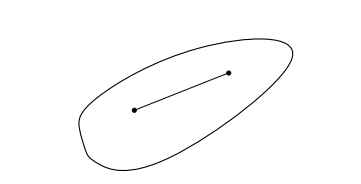
\includegraphics[width=0.8\textwidth]{figure/ch1/convex_set1.png}
        \caption{an example of a convex set}
    \end{minipage}%
    \begin{minipage}[t]{0.5\linewidth}
        \centering
        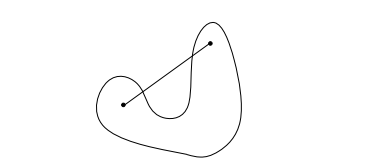
\includegraphics[width=0.8\textwidth]{figure/ch1/non_convex_set1.png}
        \caption{an example of a non convex set}
    \end{minipage}
\end{figure}


\begin{definition}{
    (Convex Function) % 定理的名字
  }{% label
  }
    {
        a function $f: \Omega \rightarrow \R$ is convex, if $\Omega$ is convex and if
         \begin{equation}
            \forall x,y \in \Omega, t\in [0,1]: f(x+t(y-x))\leq f(x)+t(f(y)-f(x)). 
         \end{equation}
    }
\end{definition}

\begin{remark}
    This definition is equivalent to saying that
    all secants are above graph.
\end{remark}


\begin{figure}[htbp]
    \centering
    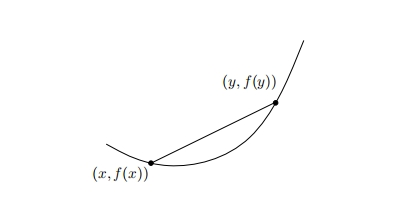
\includegraphics[width=0.6\textwidth]{figure/ch1/secant_above_graph1.png}
    \caption{For a convex function, the line segment \\ between any two points on the graph lies
    above the graph}
\end{figure}

\begin{definition}{
    (Convex Optimizaiton Problem) % 定理的名字
  }{% label
  }
    {
        an optimization problem with 
        \begin{itemize}
            \item a convex feasible set $\Omega$ and 
            \item a convex objective function $f: \Omega\rightarrow\R$
        
        \end{itemize}
        is called a "convex Optimization problem"
    }
\end{definition}

\begin{theorem}{
    (Local Implies Global Optimality for Convex Problems)
}{}
    {
        for a convex Optimization problem, every local minimum is also a global one. 
    }
\end{theorem}

\begin{proofsolution}
   
    \textcolor{LightRed}{
        Consider a local minimum $x^*$ of the convex optimization problem
        \begin{equation}
            \begin{split}
                \min_{x\in \R^n} f(x)\\
                s.t. x\in \Omega \nonumber
            \end{split}
        \end{equation}
        We will show that for each y $\in \Omega$ it holds $f(y)\geq f(x^*)$. 
    }

    Suppose that $x^*$ is not the global minmium, that is $\exists \ \widetilde{x} \in \Omega \ s.t. \ f(\widetilde{x})<f(x^*)$. \par
    Consider the line segement $x(t)=tx^*+(1-t)\widetilde{x}, t\in [0,1]$, 
        noting that $x(t)\in \Omega$ by the convexity of $\Omega$. 
        By the convexity of $f$,
        \begin{equation*}
            f(x(t))\leq tf(x^*)+(1-t)f(\widetilde{x})<tf(x^*)+(1-t)f(x^*)=f(x^*),\forall t\in [0,1]
        \end{equation*}
    \par
    As $x^*$ is a local minmium, we know that $\exists N$($N$ is a neighbourhood of $x^*$), $\forall x\in N$, $f(x)\leq f(x^*)$. 
        We can pick $t$ sufficiently to $1$ such that $x(t) \in N$. Then $f(x(t)) < f(x^*)$. 
        This is a contradiction as $f(x(t))<f(x^*)$ by the above inequality.
    \par
    Hence, $x^*$ is the global minimum. 
\end{proofsolution}

%%%%%%%%%ch1 section1 end%%%%%%%%

%%%%%%%%%ch2 section2%%%%%%%%%%%%

\section{How to Check Convexity of Functions?}

\begin{theorem}{
    (Local Implies Global Optimality for Convex Problems)
}{}
    {
        for a convex Optimization problem, every local minimum is also a global one. 
    }
\end{theorem}

%%%%%%%%

%%%%%%%%
\section{convex optimization problems}


%%%%%%%%%%%%%ch1 end%%%%%%%%%%%%%%


%%%%%%%%%%%%ch2 linear progrmming%%%%%%%

\chapter{Linear Programming}
\section{Introduction to LP}

\section{LP Relaxation}


\section{Algorithms Solving LP}



%%%%%%%%%%%%%%%%%%%%%%%%%%%%%part 2 




%%%%%%%%%%%%%%%Content%%%%%%%%%%%%%%%
% % \mainmatter % separat the number of toc and mainmatter
% \chapter*{Preface}

Notes mainly refer to following materials:


\begin{itemize}
    \item[*] Machine learning
    \begin{itemize}
        \item \href{https://www.cs.cornell.edu/courses/cs4780/2023sp/}{lecture notes from cornell}
        \item \href{https://www.cs.cmu.edu/~hn1/documents/machine-learning/notes.pdf}{lecture notes from cmu}
        \item \href{https://cs229.stanford.edu/main_notes.pdf}{lecture notes of CS229}
    \end{itemize}
    \item[*] Deep learning
    \begin{itemize}
        \item \href{https://udlbook.github.io/udlbook/}{understanding deep learning}
        \item \href{https://www.bilibili.com/video/BV1Wv411h7kN/?spm_id_from=333.337.search-card.all.click}{lecture video from Hongyi Lee}
        \item \href{https://cs231n.github.io/}{lecture notes from Stanford}
    \end{itemize}
    \item[*] Reinforcement learning
    \begin{itemize}
        \item \href{https://web.stanford.edu/class/cs234/modules.html}{lecture notes from stanford}
        \item \href{https://people.cs.umass.edu/~bsilva/courses/CMPSCI_687/Fall2022/Lecture_Notes_v1.0_687_F22.pdf}{lecture notes from umass}
    \end{itemize}
\end{itemize}








% \part{Mathematics}

% % !TEX root = ../notes_template.tex
\chapter{Discrete Math}\label{chp:discrete_math}


\section{Proof}

\begin{theorem}
\end{theorem}

\begin{solution}
By induction:
\end{solution}



\section{Quantifier}
\lipsum % dummy text - remove from real document

\section{Graph}
\citetitle{babaiGraphIsomorphismQuasipolynomial2016}
\cite{babaiGraphIsomorphismQuasipolynomial2016}

\section{Number theory}
Figure example
\begin{figure}[!ht]
    \centering
    \includegraphics[width=1\linewidth]{./figure/elliptic_curves.pdf}
    \caption{Elliptic curves \cite{childsUniversalComputationQuantum2009} }
\end{figure}


\section{Algorithm}
% \begin{center}
% \begin{minipage}{.9\linewidth}
% algorithm2e
% https://www.overleaf.com/learn/latex/Algorithms#The_algorithm2e_package
\begin{algorithm}[H]
    \SetKwInOut{Input}{input}
    \SetKwInOut{Output}{output}
    \Input{Integer $N$ and parameter $1^t$}
    \Output{A decision as to whether $N$ is prime or composite}
    \BlankLine
    \For{ $i = 1,2, \ldots, t$} {
        $a\leftarrow \qty{1,\dots,N_1}$\;
        \If{$a^{N-1} \neq 1 \mod{N}$}
    {\Return "composite"}
    }
    \Return "prime"
    \caption{Primality testing - first attempt}
    \label{alg:miller_rabin}
\end{algorithm}
% \end{minipage}
% \end{center}

% \part{Computer Science}
% % \input{./chapter/complexity.tex}
% % !TEX root = ../notes_template.tex
\chapter{Machine Learning}\label{chp:machine_learning}
\minitoc

\section{Regression}
% \gls{algorithm};
\subsection{Gradient descent}\label{sec:gradient_descent}
\gls{gd};
% \glsxtrshort{gd}

\section{Support Vector Machine}
\gls{svm};
% % \input{./chapter/algorithms.tex}

% \part{Physics}
% % !TEX root = ../notes_template.tex
\chapter{Quantum Mechanics}\label{chp:quantum_mechanics}
\minitoc

\section{Hamiltonian}
\gls{hamiltonian};
% \glsxtrshort{qm};

\section{Path Integral}
\gls{lagrangian}

\section{Quantum Field Theory}
\gls{qft};
% % \input{./chapter/quantum_field_theory.tex}

% % \begin{appendices}
% % % !TEX root = ../notes_template.tex
\chapter{Formulas}

\section{Gaussian distribution}\label{sec:gaussian_distribution}
\begin{Definition}[Gaussian distribution]\label{def:gaussian_distribution}
    \myindex{Gaussian distribution}
\end{Definition}

\begin{theorem}[Central limit theorem]\label{thm:central_limit_theorem}
\end{theorem}
% % \end{appendices}

% \backmatter

% %%%%%%%%%%%%%%% Reference %%%%%%%%%%%%%%%

% \printbibliography[heading=bibintoc]
% \printindex
\end{spacing}
\end{document}